\documentclass[%
reprint,
amsmath,amssymb,
aps,
]{revtex4-1}
\usepackage{graphicx}% Include figure files
\usepackage{dcolumn}% Align table columns on decimal point
\usepackage{bm}% bold math
\usepackage[utf8]{inputenc}
\usepackage{listings}
\usepackage{amsmath}
\usepackage{physics}
\usepackage{booktabs}
\usepackage{float}
\bgroup
\def\arraystretch{1.3}
\newcommand{\HRule}{\rule{\textwidth}{0.5mm}}
\makeatletter
\newcommand*{\rom}[1]{\expandafter\@slowromancap\romannumeral #1@}
\makeatother

\begin{document}
\onecolumngrid

\begin{center}
	\large\textbf{Numerical integration methods\\ \small{The Gaussian Quadrature and Monte Carlo Procedures}}
\end{center}
\vspace{5mm}

\begin{center}
	\small{$^1$ Oline A. Ranum}\\
\end{center}

\begin{center}
	\small{$^1$ University of Oslo, Institute of physics, 
		olinear@student.matnat.uio.no}
\end{center}

\begin{center}
	\textit{\today}
\end{center}
\vspace{7mm}
\noindent 
\HRule \\
In this numerical experiment the numerical integration of the expectation value of the exchange energy between two electrons in a helium atom, $E[f]$, is estimated using both the Gaussian Quadrature and Monte Carlo integration. The integral is estimate using a Gauss-Legendre procedure yielding $E[f] \approx (1.9 \pm 0.2)$ and a Gauss-Laguerre procedure yielding $E[f]\approx (1.9 \pm 0.1)\times 10^{-1}$. The error is taken to be the relative error. The estimates are compared with the exact value for $alpha = 2$ that is $I = 1.928\times 10^{-1}$. A brute force Monte Carlo method finds the value and variation $E[f]\approx (1.8983 \pm 0.0003)\times 10^{-1}$ based on a uniform distribution. An improvement to this estimate using importance sampling finds the value $E[f]\approx (1.9292 \pm 0.0004)\times 10^{-1}$. In the end, the importance sampling is parallelized and set to run on four processors, yielding $E[f]\approx (1.9264 \pm 0.0004)\times 10^{-1}$ with a grater potential for efficiency. It is concluded that a parallelized Monte Carlo integration with importance sampling is the most efficient method, as well as yielding the highest accuracy. 
  \\
\HRule
\vspace{1cm}

\section{Introduction}
\vspace{3mm}
\twocolumngrid 
Wherever you go in modern day science, there is a need for approximating integrals where an exact solution has not yet been established. Numerical integration is a term that first occurred in the 20th century. It has since become one of the most valuable tools in modern day science, and a widely studied subject. Amongst some of the most famous and useful approaches to numerical integration is both the Gaussian Quadrature and Monte Carlo Integration. I will in this paper investigate both of these approaches to solve for the expectation value of the ground state correlation energy between two electrons in a helium atom. \\
\indent The papers initially presents all necessary theory for the experiment, and goes through the methods applied. The integral is first estimated using a Gauss-Legendre procedure, followed by an approach using Gauss-Laguerre. Thereafter, a brute force Monte Carlo integration is implemented using a uniform distribution function. The Monte Carlo approach is then improved implementing importance sampling and parallelization. The results are presented and discussed in regards to both efficiency and accuracy. A conclusion is presented on the back of the discussion, and states that the Monte Carlo method was found preferable for the above purpose. \\
Monte Carlo methods are widely used in Science, from integration of multi-dimensional integrals to solving ab initio problems in for instance chemistry, physics, medicine or biology. The Gauss quadrature yielding an alternative approach to solve for some of these problems, presents the opportunity for discussion around both efficiency and accuracy in our methods. Numerical integration is a rich field that continuous to grow, and exaclty because of that this paper is important in regards to understanding the various components and contributions of our methods. A more thourough understanding of our methods leads to new fields and application, like for instance the finding of applying Monte Carlo methods into the newly upcoming field of computational science. I hope that this paper will be a contribution to a more thorough understanding of Monte Carlo integration as well as the Gaussian Quadrature. \newpage 
 
\section{Theory}



\subsection{Numerical integration \& the Gaussian quadrature} \noindent 
The basic idea behind all numerical integration methods is to approximate the integral 
\begin{equation}\label{numint}
	I = \int_{a}^{b}f(x)dx \approx \sum_{i=0}^{N-1} \omega_if(x_i)
\end{equation}
where $\omega$ and $x$ are the weights and the chosen mesh points, respectively. Interpolatory quadrature rules, such as Simpson's- or the trapezoidal rule, are based on the assumption that the quadrature points, or nodes, are preassigned equidistantly or with a fixed distribution. The Gaussian quadrature (hereafter GQ) is based on the notion first made by Gauss, that a suitable variation of the nodes would in general lead to a better accuracy [Kythe \& Schaferkotter, 2005]. The core idea of GQ is to have the freedom to choose both the weighting coefficients and the location of the abscissas/nodes at which the function is to be evaluated. One therefore no longer requires the nodes to be equally spaced, and therefore giving twice the number of degrees of freedom in regards to the classical interpolatory quadratures [Press et al. 2007]. As such, many variations and generalizations of the Gaussian formulas have been developed on the form equation \ref{numint}, where the weights $\omega_i$ are positive zeros of certain orthogonal polynomials and the nodes $x_i$ are distinct points in a given interval [Kythe \& Schaferkotter, 2005]. \\
\indent It is important to note that higher order does not necessarily imply higher accuracy. The former only implies the latter in the case where the integrand is very smooth, in the sense that the integrand is well approximated by a polynomial. In the case of a Gaussian quadrature, it is possible to arrange both weights and abscissas to make integrals exact for a class of integrands on the form of polynomials times some known function $W(x)$. One chooses $W(x)$ to remove integratable singularities from the desired integral. As stated in Press et al., given $W(x)$ and an integer N, it is possible to find a set of weights $w_j$ and nodes $x_j$ such that the approximation 
\begin{equation}
	\int_{a}^{b}W(x)f(x)dx \approx \sum_{j = 0}^{N-1}w_jf(x_j)
\end{equation}
is exact if $f(x)$ is a polynomial. [Press et al., 2015]


\subsection{Orthonormal polynomials} \noindent 
The subject of Gaussian quadratures was further developed by Jacobi's derivation of Gauss's work by means of orthogonal polynomials [Press et al. 2007]. A set of polynomials $\{p_i\}$ of degree $i$ is said to be orthogonal with respect to the inner-product if $<p_i, p_j> = 0$ for $i\not = j$ on a finite or infinite interval $[a,b]$. That is, if the powers are orthonormalized, one should obtain a unique set of polynomials $p_i(x)$ of degree $n$ such that
\begin{equation}
	\braket{p_i}{p_j} = 
	\int_{a}^{b} W(x)p_i(x)p_j(x)dx = \delta_{ij} 
\end{equation}
where $\delta_{ij}$ is the Kronecker delta
\begin{equation}
	\delta_{ij} = \left\{
	\begin{array}{ll}
	1 & i = j\\
	0 & i \not =j 
	\end{array} \right\}
\end{equation}
The orthogonality property for polynomials defined in this manner is equivalently defined for a discrete set of polynomials [Kythe \& Schaferkotter, 2005]. Two functions are said to be normalized if its scalar product with itself is unity. A set of functions that are all mutually orthogonal and also all  individually normalized is called an orthonormal set.  [Press et al., 2015]

\subsubsection{Constructing orthogonal polynomial sets}
It is possible to find a set of polynomials through recurrence relations which has the property of beeing mutually orthogonal over a spesified weight function W(x) and that includes exactly one polynomial of order $j$, called $p_j(x)$ for each $j = 0,1,2,\dots$. Such a constructive procedure is described by Press et al.:
\begin{align*}
	p_{-1}(x) &\equiv 0\\
	p_{0}(x) &\equiv 1\\
	p_{j+1}(x) &\equiv (x-a_j)p_j(x)-b_jp_{j-1}(x)\\
\end{align*}
where
\begin{align*}
	a_j &= \dfrac{\braket{xp_j}{p_j}}{\braket{p_j}{p_j}} &\hspace{1mm} j = 0,1, \dots \\ &&\\
	b_j &=\dfrac{\braket{p_j}{p_j}}{\braket{p_{j-1}}{p_{j-1}}} &\hspace{1mm} j = 1,2, \dots
\end{align*}
The coefficient $b_0$ would be arbitrary, and can therefore be set to zero. It can be showen that the polynomial $p_j(x)$ have exactly $j$ distinct roots in a given interval $[a,b]$. \\
The fundamental theorem of Gaussian quadratures then states that the  abscissas of the N point Gaussian quadrature equations with weighting function W(x) in the interval $[a,b]$ are precisely the roots of the orthogonal polynomial $p_N(x)$ for the same interval and weighting function. Once the abscissas are known, one needs to find the weights $w_j$. For classical orthogonal polynomials, such as the Gauss-Legendre and Gauss-Laguerre, the coefficients $a_j$ and $b_j$ have an explicit solution. Thus, the problem reduces to determining the zeros of the polynomial $p_N(x)$, and the computation of the weights [Press et al.]\\

\subsubsection{Computation of abscissas and weights}
Both the Gauss-Legendre and - Laguerre are classical, well-studied, orthogonal polynomials and can be used as good starting guesses. After an initial guess is made, one can apply Newtons method, and expect  it to converge rather rapidly to locate the zero-point. [Press et al.] \\
For the Gauss-Legendre and Gauss-Laguerre the following direct root finding is concidered to be faster by a factor of 3 to 5, than any other method [Press et al.]\\
\textit{Gauss-Legendre}:
\begin{equation*}
	W(x) = 1 \hspace{3mm} -1 < x < 1 
\end{equation*}
\begin{equation}\label{glegfunc}
	(j+1)P_{j+1} = (2j +1)xP_j - jP_{j-1}
\end{equation}
\textit{Gauss-Laguerre}
\begin{equation*}
W(x) = x^\alpha e^{-x} \hspace{3mm} 0 < x < \infty 
\end{equation*}
\begin{equation}
(j+1)L_{j+1}^\alpha = (-x+2j+\alpha+1)L_j^\alpha -(j+\alpha)L_{j-1}^\alpha
\end{equation}
\subsubsection{The Newton-Raphson method} \noindent 
The Newton-Raphson method is a one-dimensional root-finding routine, that easily generalizes to multiple dimensions. The method requires the evaluation both of the function and the derivative of the function, at arbitrary points x. The method is geometrically an extension of a tangent line at the current point $x_i$ until the tangent crosses zero, then setting the next guess $x_{i+1}$ to the abscissa of that zero crossing. The method derives from a Taylor series expansion of a function in the neighborhood of a point. The Newton-Rapson formula is expressed as
\begin{equation}
	x_{i+1} = x_i -\dfrac{f(x_i)}{f'(x_i)}
\end{equation}
with associated error propagation
\begin{equation}
	\epsilon_{i+1} = \epsilon_i  -\dfrac{f(x_i)}{f'(x_i)}
\end{equation}
This method is efficient as it converges quadratically. The derivate of the polynomial can be evaluated using the standard relations in terms of $p_N$ and $p_{N-1}$.  [Press]
\begin{equation}
	f'(x) \approx \dfrac{f(x+dx)- f(x)}{dx}
\end{equation}


\newpage
\subsection{Stochastic Monte-Carlo Integration}
Monte Carlo integration evaluates a function $f(x)$ at a random sample of point and estimates its integral based on that random sample. The fundamental theorem of Monte Carlo integration gives an estimate of the integral of the function over a multidimensional volume V
\begin{equation}
	\int f dV \approx V \langle f\rangle \pm V\sqrt{\dfrac{ \langle f^2 \rangle - \langle f \rangle^2}{N}}
\end{equation}
The $\pm$-term is the one standard deviation error estimate for the integral. The angle brackets denote taking the arithmetic mean over the N sample points 
\begin{equation}
	\langle f \rangle \equiv \dfrac{1}{N}\sum_{i=0}^{N-1}f(x_i)
\end{equation}
\begin{equation}
\langle f^2 \rangle \equiv \dfrac{1}{N}\sum_{i=0}^{N-1}f^2(x_i)
\end{equation}
[Press et al. ]

\subsubsection{Probability distribution functions}
The only requirement for many applications of Monte Carlo methods is that a probability distribution function (PDF) is known to describe the physical system. Once a PDF is known a Monte Carlo simulation can proceed by random sampling from the PDF's. 

Since the result is built on the average of many simulations over the number of ovservations, the statical error - the variance - can be predicted. The PDF is a function $p(x)$ on the domain which in the discrete case gives us the probability or relative frequency with which these values of X occure 
\begin{equation}
	p(x) = \textnormal{Prob}(X=x)
\end{equation}
The PDF must satisfy two properties. First, the PDF has tobe nprmalized so that all the probabilities add up to unity
\begin{equation}
	\sum_{x_i\in \mathcal{D}} p(x_i) = 1
\end{equation} 
Assuming that the PDF is normalized, the probability then has to be of a positive nature 
\begin{equation}
	0 \leq p(x) \leq 1
\end{equation}
One especially important PDF is the uniform distribution defined as 
\begin{equation}\ref{unipdf}
	p(x) = \dfrac{1}{b-a}\Theta(x-a)\Theta(b-x)
\end{equation}
where
\begin{align*}
	\Theta(x) &= 0& \hspace{2mm} x < 0\\
	\Theta(x) &= 1& \hspace{2mm} x \geq 0\\
\end{align*}
Another important probability distribution is the exponential distribution 
\begin{equation}\label{exppdf}
	p(y) = \exp{-y}
\end{equation}
where $p(x)$ is given by the uniform distribution $x\in[0,1]$. Assuming that the probability is conserved through the variable transformation
\begin{equation}
p(y)dy = \exp{-y}dy = dx
\end{equation}
The above definitions is written as functions of a single stochastic variable, and is thereby known as univariante. A PDF consisting of multiple variables is usually refered to as mutlivariante, and the multivariante expectation value is defined similarly as the above univariante case, but all stochastiv variables are taken into account simultaniously on the form
\begin{equation}
	E[f(x_1\dots x_N)] = \int\dots\int f(x_1\dots x_N)P(x_1\dots x_N)dx_1\dots dx_2
\end{equation}
In the case where the variables are uncorrelated, the factor P can be factorized in the following form
\begin{equation}
	P(x_1,\dots,x_N) = \prod_{i = 1}^{N} p_i(x_i)
\end{equation}
where $p_i(x_i)$ is the univariant PDF of $X_i$.


\subsubsection*{The Monte Carlo method} \noindent 
Given the above definition of the PDF and taking the weights of the integral definition from equation \ref{numint} to be equal to one, $\omega_i = 1$, one gets the corresponding rectangle method
\begin{equation*}
I = \int_{a}^{b}f(x)dx \approx h\sum_{i=1}^{N}f(x_{i-1/2})
\end{equation*} 
where $f(x_{i-1/2})$ is the midpoint value of f for a given value $x_{i-1/2}$. Using $h = (b-a)/N$ where $b=1$ and $a=0$ the integral can be expressed as
\begin{equation*}
I = \int_{0}^{1}f(x)dx \approx \dfrac{1}{N}\sum_{i=1}^{N}f(x_{i-1/2})
\end{equation*} 
Then the average of the function f for a given PDF $p(x)$ is
\begin{equation}\label{mcint}
\langle f \rangle = I = \int_{a}^{b}f(x)P(x)dx \approx \dfrac{1}{N}\sum_{i=1}^{N}f(x_i)p(x_i) 
\end{equation}
[M. Jensen]

\subsubsection{Monte Carlo Error}
For a stochastic variable X, the variance $Var(X) = \sigma_X^2 $
\begin{align}\label{var}
	Var(x) = \sigma_X^2 &= \expval{(x-\expval{x})^2} c\nonumber \\
	&= \int(x-\expval{x})^2p(x)dx\nonumber\\
	&= \int(x^2-2x\expval{x}^2+ \expval{x}^2)p(x)dx\nonumber\\
	& = \expval{x^2} - \expval{x}^2
\end{align}
[Press]



\subsubsection{Importance sampling}
Importance sampling is based on a change of variables $p(x)\rightarrow p(y)$ in the case that a probability distribution function $p(y)$ follows F closely. This is useful as this leads to a smooth integrand where it is possible to sample over the relevant values for the integrand. In the case that $p(y)$ is a normalized PDF whose behavior resembles that of a function F defined in a certain interval [a, b], the integral can be rewritten as 
\begin{equation}
	I = \int_{a}^{b}F(y)dy = \int_{a}^{b}p(y)\dfrac{F(y)}{p(y)}dy 
\end{equation}
when $x\in[0,1]$ are a uniform distribution of random numbers, one preformes a change of variables $x\rightarrow y$ through
\begin{equation}
	x(y) = \int_{a}^{y}p(y')dy'
\end{equation}
where
\begin{equation}
	p(x)dx = dx = p(y)dy
\end{equation}
then the inverted of $x(y)$ will be $y(x)$. Thus
\begin{equation}
I = \int_{a}^{b}p(y)\dfrac{F(y)}{p(y)}dy  = \int_{a}^{b}\dfrac{F(y(x))}{p(y(x))}dx
\end{equation}
Yielding the following Monte Carlo evaluation 
\begin{equation}
	\int_{\bar{a}}^{\bar{b}}\dfrac{F(y(x))}{p(y(x))}dx = \dfrac{1}{N}\sum_{i=1}^{N}\dfrac{F(y(x_i))}{p(y(x_i))}
\end{equation}
where $\bar{a}$ and $\bar{b}$ are the transformed integration limits. It is non-trivial to find such a function $p$, and the transformations are restricted to the case where $p$ is normalizable and positive definite, analytically integrable and the integral is invertible. The variance after such a transformation will be given as 

\begin{equation}
	\sigma^2 = \dfrac{1}{N}\sum_{i = 1}^{N}\qty(\dfrac{F(y(x))}{p(y(x))})^2 -\qty(\dfrac{1}{N}\sum_{i = 1}^{N}\dfrac{F(y(x))}{p(y(x))})^2
\end{equation}
\subsection{Parallelization}
\newpage 
\subsection{The wave-function for a helium atom} \noindent 
The single-particle wave function for an electron $i$ in the $1s$ state is given in terms of a dimensionless variable 
\begin{equation*}
	 {\bf r}_i =  x_i {\bf e}_x + y_i {\bf e}_y +z_i {\bf e}_z 
\end{equation*}
as 
\begin{equation*}
	\psi_{1s}({\bf r}_i)  =   e^{-\alpha r_i},
\end{equation*}
where $\alpha$ is a parameter and 
\begin{equation*}
	r_i = \sqrt{x_i^2+y_i^2+z_i^2}
\end{equation*}
For a helium atom, $\alpha = 2$ corresponds to the charge of the atom $Z = 2$. The ansatz for the wave function for a two electron system in a helium atom is then assumed to be given by the product of two such 1s wave functions, 
\begin{equation}\label{waveequation}
	\Psi({\bf r}_1,{\bf r}_2)  =   e^{-\alpha (r_1+r_2)}
\end{equation}
This ansatz does not yield a closed-form or analytical solution to Schrodinger's equation for two interacting electrons in the helium atom. \\ \indent 
To find the ground state correlation energy between the two electrons, one looks to the following six-dimensional integral yielding the quantum mechanical expectation value of the correlation energy between two electrons which repel each other via the classical Coulomb interaction
\begin{equation}\label{ccintegration}
	   \langle \frac{1}{|{\bf r}_1-{\bf r}_2|} \rangle =
	\int_{-\infty}^{\infty} d{\bf r}_1d{\bf r}_2  e^{-2\alpha (r_1+r_2)}\frac{1}{|{\bf r}_1-{\bf r}_2|}
\end{equation}
This wave function is not normalized, but the integral has the closed form solution for $\alpha = 2$
\begin{equation*}
\langle \frac{1}{|{\bf r}_1-{\bf r}_2|} \rangle = \dfrac{5}{16^2}\pi^2
\end{equation*}
See appendix for the derivation of this value. 
\subsubsection*{Note on numerical integration of the wave function} \noindent 
In the case that integral \ref{ccintegration} is evaluated numerically, one must consider the approximation to the integration limits. For a wave function on the form of an exponential function, the function will often converge quickly towards zero. Thus, for all practical purposes, the lower- and upper integration limits in integral \ref{ccintegration} can be substituted by a finite number $\pm \lambda$. \\
Furthermore, in the case of evaluation by a Gauss-Legendre quadrature it is possible to use Cartesian coordinates and evaluate integral \ref{ccintegration} directly. On the other hand, if Gauss-Laguerre quadrature is applied, a transformation into polar-coordinates might be necessary.
\subsubsection*{Transformation to polar coordinates}  
Laguerre polynomials are defined for $x\in[0,\infty)$, and expressed in polar coordinates. To translate integral \ref{ccintegration} into a spherical coordinate system one employs the following relations

\begin{equation*}
	d{\bf r}_1d{\bf r}_2  = r_1^2dr_1 r_2^2dr_2 dcos(\theta_1)dcos(\theta_2)d\phi_1d\phi_2,
\end{equation*}
with
\begin{equation*}
	\frac{1}{r_{12}}= \frac{1}{\sqrt{r_1^2+r_2^2-2r_1r_2cos(\beta)}}
\end{equation*}
and 
\begin{equation}
	cos(\beta) = cos(\theta_1)cos(\theta_2)+sin(\theta_1)sin(\theta_2)cos(\phi_1-\phi_2))
\end{equation}
yielding the integral expressed as \\ 
\begin{align}\label{cpintegration}
	\langle \frac{1}{\abs{{\bf r}_1-{\bf r}_2}} \rangle =& \nonumber \\ 
	\int_{0}^{\infty}\int_{0}^{\infty}\int_{0}^{2\pi}\int_{0}^{2\pi}\int_{0}^{\pi}\int_{0}^{\pi}
	r_1^2dr_1 r_2^2dr_2 dcos(\theta_1)dcos(\theta_2)d\phi_1d\phi_2 & \nonumber \\ 
	\times e^{-2\alpha (r_1+r_2)}\frac{1}{\sqrt{r_1^2+r_2^2-2r_1r_2cos(\beta)}}
\end{align}


\vspace{10mm}
\newpage 
\section{Method}\noindent 
I will in this paper estimate the quantum mechanical expectation value of the correlation energy between two electrons which repel each other via the classical Coulomb interaction as given in equation \ref{ccintegration} using a selection of numerical integration methods. I will initially exploit a Gauss-Legendre approach, then a further development using a Gauss-Laguerre approach and in the end I will investigate a Monte Carlo integration over the system. 
\subsubsection*{The ground state wave equation} \noindent 
Initially a plot is produced of the ground state wave equation for a two electron system, as described by equation \ref{waveequation}. The plot is then used to determine the appropriate integration limits $\pm \infty \rightarrow \pm \lambda$ for evaluation of integral \ref{ccintegration}, and $\lambda = 2$ is set for the duration of this paper.  

\subsection{Integration using Gauss-Legendre Quadrature}\noindent 
I initially apply a Gauss-Legendre quadrature to compute the six dimensional integral over all Cartesian spatial variables. The integration is carried out using the weighting function and recurrence relation as presented in equation set \ref{glegfunc}, and is based on the classical Legendre polynomials as presented in the appendix. I evaluate the integral for a selection of N values, consisting of $N = 2n+1 \hspace{2mm} \forall \hspace{2mm}n\in[4,19]$. The results are plotted and presented in the result section. Tabulated values are presented in the appendix. Only odd values of N are used on the basis of the symmetry of the roots. The case of  $\abs{\mathbf{r_1} -\mathbf{r_2}} = 0$ is discharged from the integral, and not taken into consideration. The integration procedure is based on the procedure outlined in Press et al. [Press et al., 2007].

\subsection{Integration using Gauss-Laguerre Quadrature} \noindent 
I then developed the procedure by a transformation of integral \ref{ccintegration} into polar coordinates as presented in integral \ref{cpintegration} and I employed the Laguerre polynomials as presented in the appendix. I set the new integration limits $\theta_i \in [0,\pi]$, $\phi_i \in [0,2\pi]$ and $r_i\in[0,\infty]$. The integral is evaluated for the same range of N as the former procedure, and the algorithm is based on the same procedure as above [Press et al., 2007].

\subsection{Monte Carlo Integration}
I apply a brute-force Monte Carlo integration as defined by equation \ref{mcint}. I apply a Mersenne Twister pseudo-random generator of 64-bit numbers with a state size of 19937 bits to generate canonical random positions. I use a Cartesian abscissas system, and estimate the integral using the uniform distribution function as defined in equation \ref{unipdf}. I estimate the integral as a function of the N, and evaluate the results. I employ the same random number generator, but the positional elements are now scaled in accordance to the spherical system. The variance is estimated in accordance to equation \ref{var}.

\subsubsection*{Importance sampling}\noindent 
The procedure is improved by applying importance sampling. That includes a transformation to spherical coordinates and applying an exponential PDF as described by equation \ref{exppdf}. The variance is again estimated in accordance to equation \ref{var}. I look at the CPU time compared with that of the previous Cartesian, uniform distribution.


\subsubsection*{Parallelization of procedure}
I then use MPI to parallelize the procedure, and divide the samples on 4 processors. I employ various complier flags and comment on the results.

\newpage . \newpage
\section{Result} \noindent 
The ground state wave function for a two-electron system is plotted in figure \ref{wavefigure}. The wave function appears to have converged to zero at $r = \pm 1$. \\ \indent 
The results of the Gauss-quadrature based integration are presented in figure \ref{integrated_results}, who shows the expectation value estimate as a function of mesh points N. The time is indicated by the color gradient of the plot. The time as function of N is given explicitly in the appendix in figure \ref{itegrated time}for further details, alongside all tabulated values. The relative error is tabulated in the appendix as well, and follows the same function form as the expectation value and decreases as a function of N. The estimate of the expectation value integral appears to be converging towards values slightly diverging from exact value. It never fully approximates the solution for the selection of N values with three leading digits. The closest value for the Gauss-Legendre process is given by N = 27 converging slightly below and for Gauss-Laguerre at N = 15 converging slightly above the exact value.  

\newpage 
\begin{figure}[!ht]
	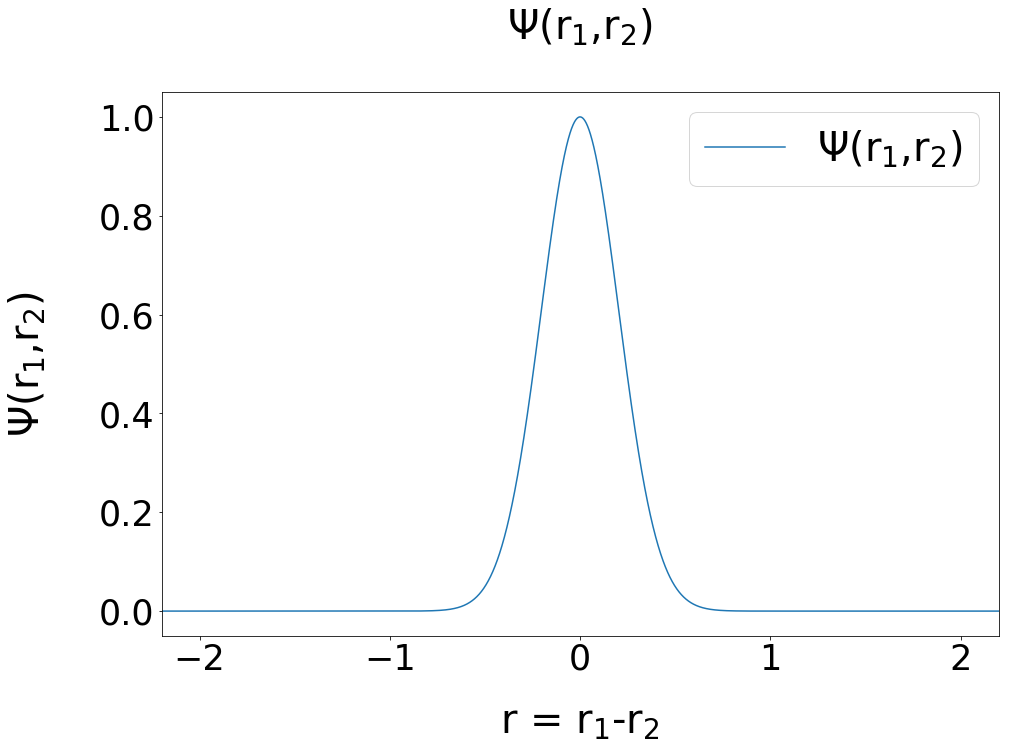
\includegraphics[scale = 0.24]{Wavefunction.png}
	\caption{\label{wavefigure} The wave function or two electrons as the product of two 1s states. The function appears to have converged to zero at r = $\pm$1 for all practical purposes.}
\end{figure}
\vspace{20mm}
\onecolumngrid

\begin{figure*}[hb!]
	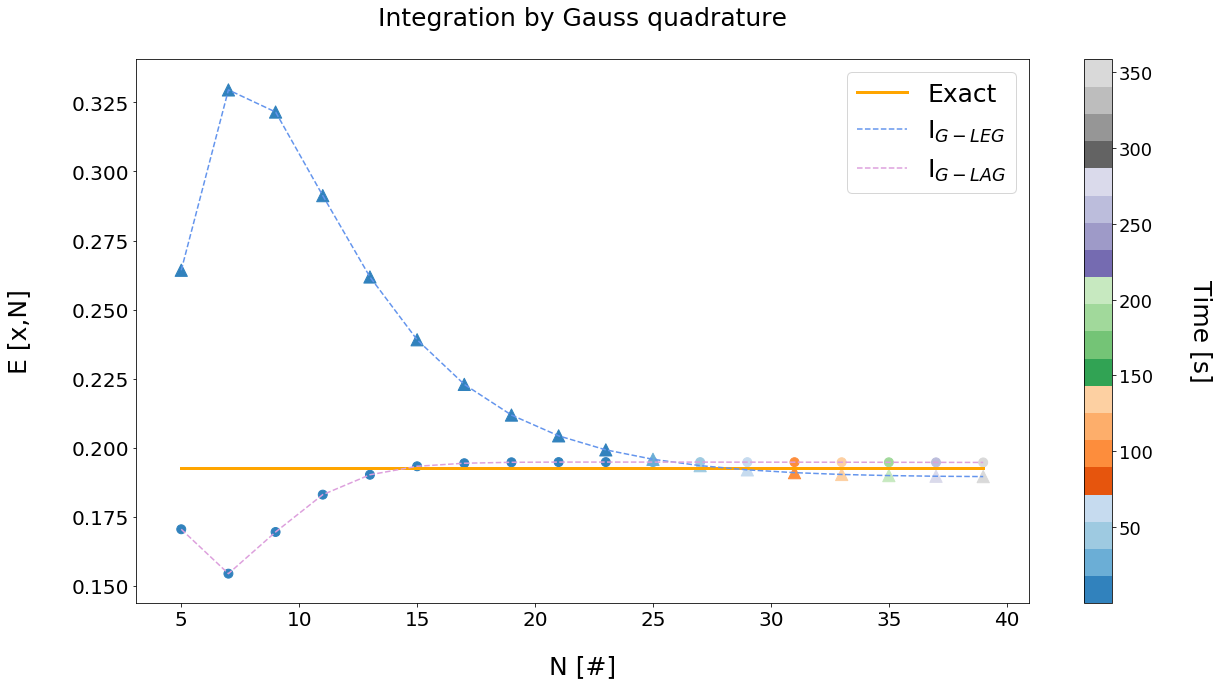
\includegraphics[width=\textwidth]{Gauss_lagleg_2.png}
	\caption{\label{integrated_results} The result of the Gauss-Legendre and Gauss-Laguerre procedures to approximate the expectation value for the interaction energy, as a function of N and the chosen x-range of $\lambda \in[-3,3]$. The exact result is $1.9277\times 10^{-1}$. }
\end{figure*}

\newpage 
\twocolumngrid
The results of the Monte Carlo integration procedures are presented in figure \ref{mc}. It is evident that the importance sampling and parallelized code produces the qualitatively best approximations. The importance sampling results are on average the closest to the exact value, but for every increase in N the approximations appears to converge closer to the exact solution.  \\  \indent 
Looking at figure \ref{mc_time} representing the time evolutions as a function of N, it is evident that the parallelized procedure of the importance sampling is significantly faster than the procedure only running on a single  processor.  Figure \ref{mc_err} gives an indication of the variance of the various Monte Carlo procedures, and figure \ref{mc_pt} shows the precision as a function of time, $t(N)$. The variance converge towards zero as N increases for all three procedures. The parallelized Monte Carlo method has initially the highest variance, followed by the brute force importance sampled procedure and then the uniform distribution based procedure. 
\\ \newpage 
\begin{figure}[H]
	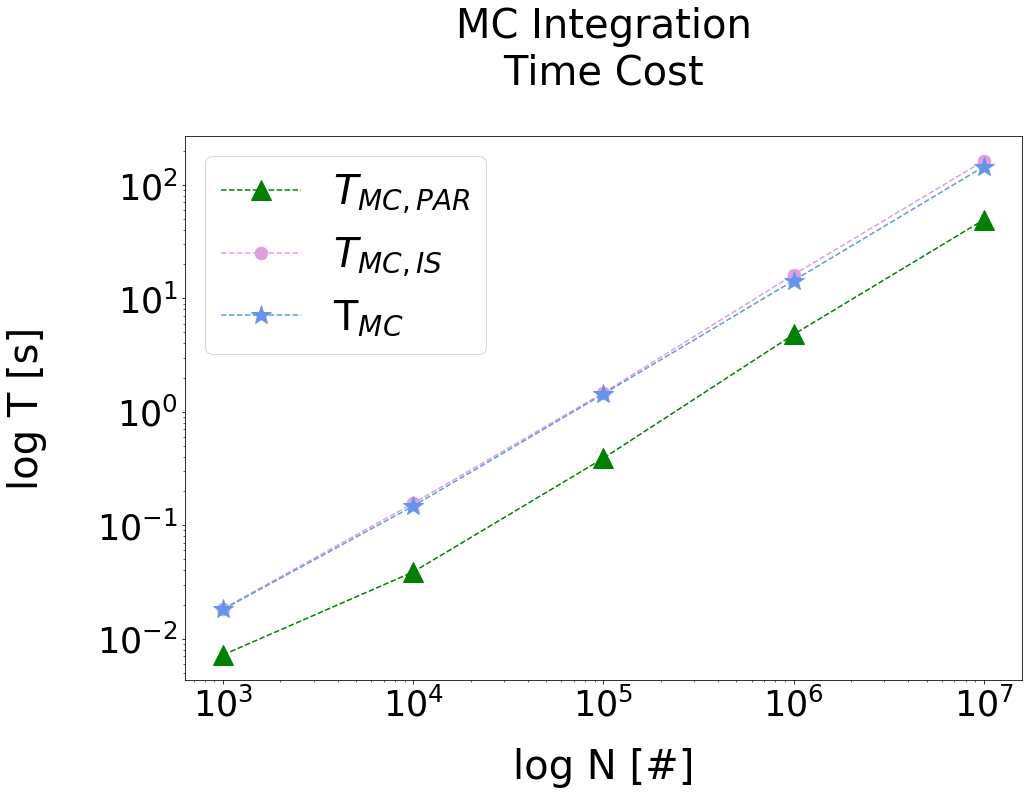
\includegraphics[scale = 0.2]{MC_time.png}
	\caption{\label{mc_time} The time result of the Monte Carlo integration procedures to approximate the expectation value of the interaction energy, as a function of N. The brute force Monte Carlo are represented by the stars, the importance sampling by the circles and the parallelized results by the triangles. }
\end{figure} 

\onecolumngrid

\begin{figure*}[!h]
	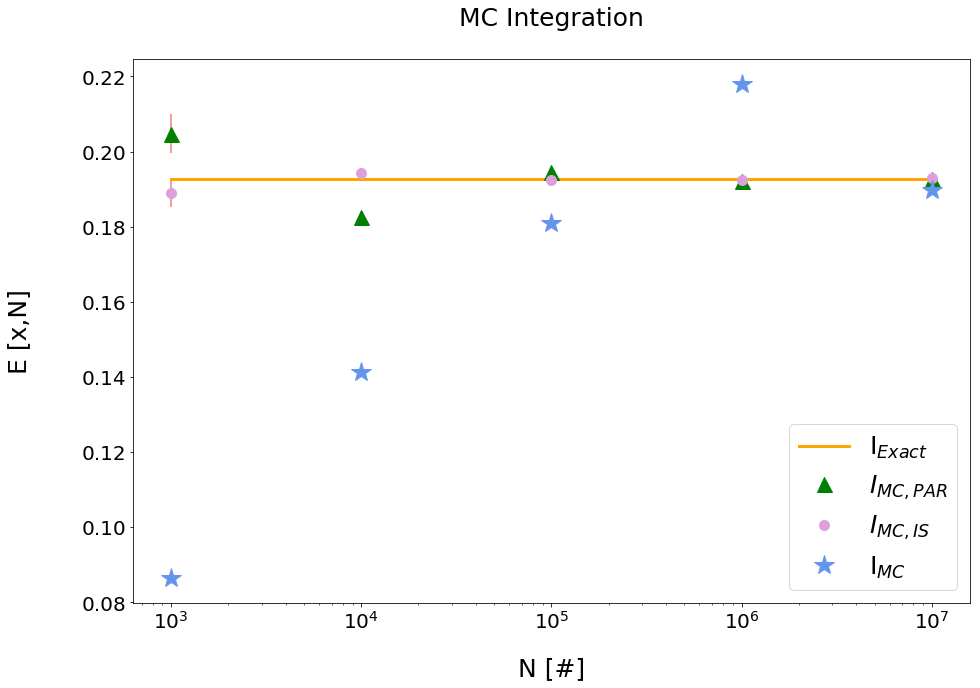
\includegraphics[width=\textwidth]{MC_integration.png}
	\caption{\label{mc_err} The result of the Monte Carlo integration procedures to approximate the expectation value for the interaction energy, as a function of N and the chosen x-range of $\lambda \in[-3,3]$. The results from the brute force Monte Carlo are represented by the stars, the results from the importance sampling are represented by the circles and the parallelized results by the triangles. The exact result is $1.9277\times 10^{-1}$. }
\end{figure*}

\begin{figure*}[!h]
	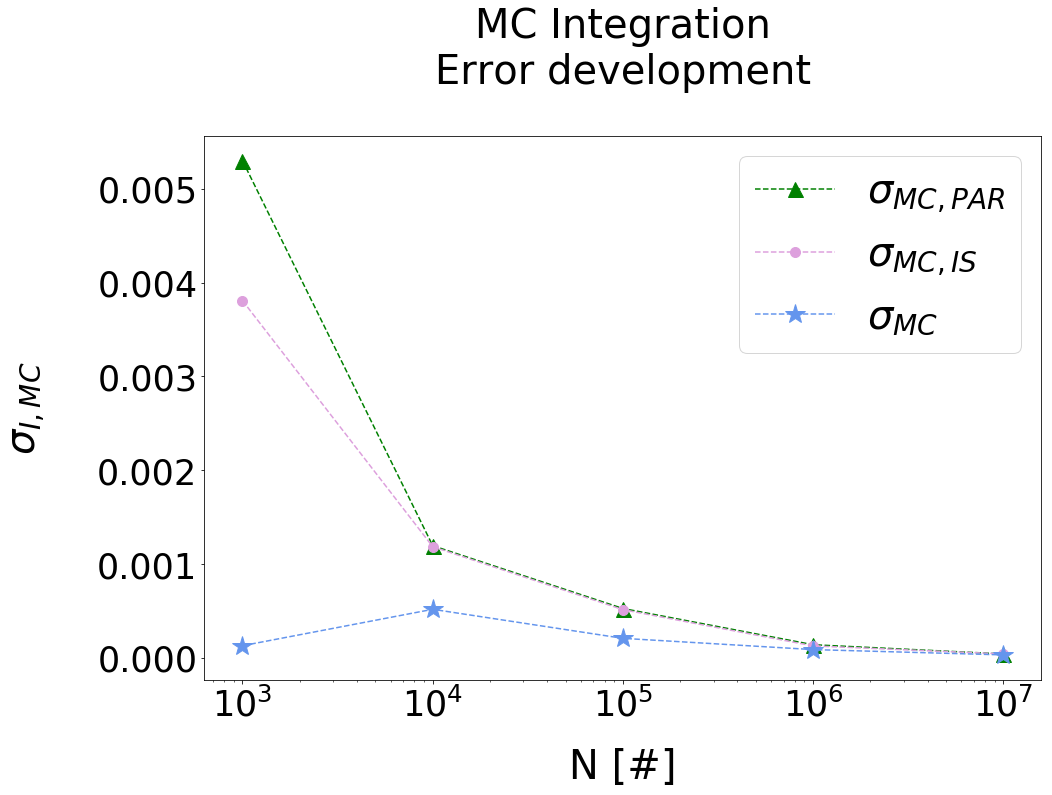
\includegraphics[scale = 0.33]{MC_integration_error.png}
	\caption{\label{mc_pt} The result of the Monte Carlo integration procedures to approximate the expectation value for the interaction energy, as a function of N and the chosen x-range of $\lambda \in[-3,3]$. The results from the brute force Monte Carlo are represented by the stars, the results from the importance sampling are represented by the circles and the parallelized results by the triangles. The exact result is $1.9277\times 10^{-1}$. }
\end{figure*}

\begin{figure*}[!h]
	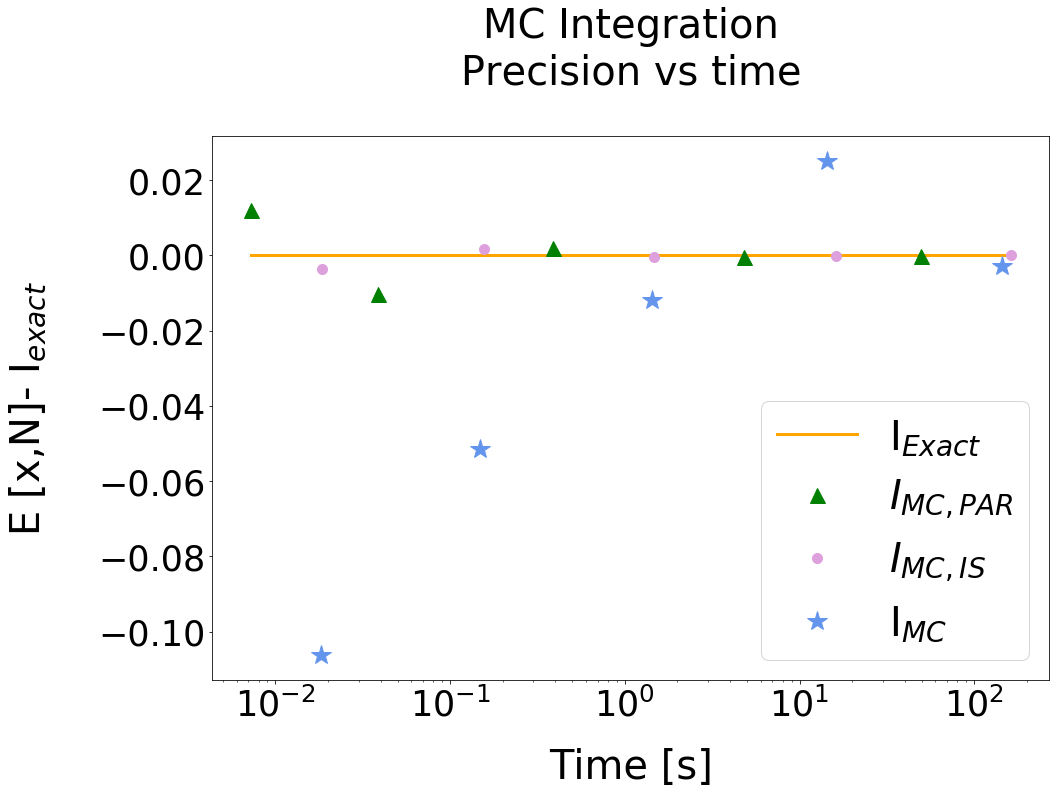
\includegraphics[scale = 0.33]{MC_integration_PT.png}
	\caption{\label{mc} The result of the Monte Carlo integration procedures to approximate the expectation value for the interaction energy, as a function of N and the chosen x-range of $\lambda \in[-3,3]$. The results from the brute force Monte Carlo are represented by the stars, the results from the importance sampling are represented by the circles and the parallelized results by the triangles. The exact result is $1.9277\times 10^{-1}$. }
\end{figure*}
\twocolumngrid
\newpage.
\newpage.
\newpage.
\newpage.
\newpage 
\section{Discussion}
In regards to the chosen $\pm \lambda$ integration limits, the results seems reasonable. A way of thesting this is ofcourse to run the program for a various selection of $\lambda$ values and map how it affects the finite results. This is deemed excessive for the purposes of this paper, and is left for future work. 
Why the results appears to converge to the wrong number, or perhaps a saddle point, is yet to be disclosed. It might be an error made in the coding, or it might be caused by a fault of method. 
\section{Conclusion }

\newpage. \newpage
\onecolumngrid
\section{Referances}
[1] Handbook of computational methods for integration, P. K. Kythe and M. R. Schaferkotter, Chapman \& Hall/CRC, Boca Raton Florida, 2005.
\newpage 
\section{Appendix}
\subsection{Time of Legendre and Laguerre procedures }
\begin{figure}[!h]
	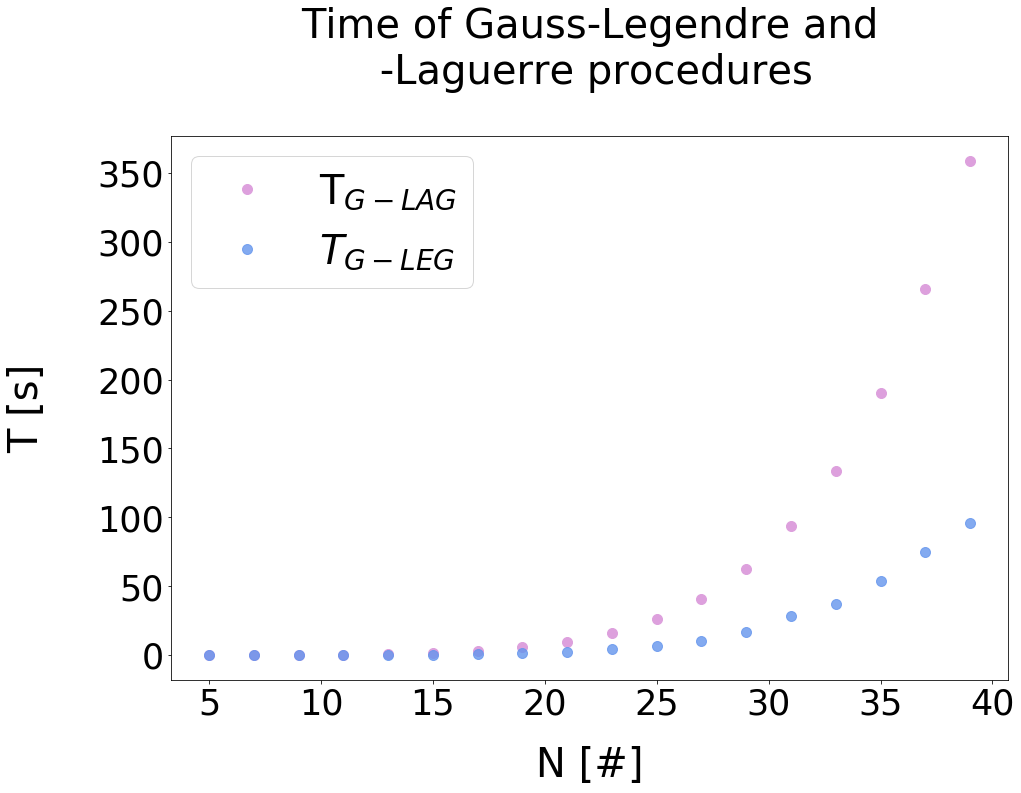
\includegraphics[scale = 0.3]{Gauss_time.png}
	\caption{\label{integrated_time} The result of the Gauss-Legendre integration as a function of N. The exact result is $1.9277\times 10^{-1}$. }
\end{figure}

\subsection{Tabulated values}

\begin{table}[!h]
	\caption {Gauss-Legendre Quadrature} 
	\begin{tabular}{|c|c|c|c|}
		\hline 
		\hspace{5mm} \textbf{N} \hspace{5mm} & \textbf{Integrated value $\times 10^{-1}$} & \hspace{3mm}\textbf{Relative error $\times 10^{-1}$} & \hspace{3mm}\textbf{Time  [s]} \hspace{5mm}\\
		\hline 
			5 & 2.642  & 4  & 0.0009 \\
			7 & 3.295  & 7  & 0.0063 \\
			9 & 3.215  & 7  & 0.0218 \\
			11 & 2.913  & 5  & 0.0572 \\
			13 & 2.618  & 3  & 0.1633 \\
			15 & 2.391  & 2  & 0.3104 \\
			17 & 2.229  & 2  & 0.6593 \\
			19 & 2.118  & 1  & 1.3405 \\
			21 & 2.043  & 0.6  & 2.4468 \\
			23 & 1.992  & 0.3  & 4.1460 \\
			25 & 1.958  & 0.2  & 6.5590 \\
			27 & 1.935  & 0.04  & 10.4028 \\
			29 & 1.920  & 0.04  & 16.5082 \\
			31 & 1.910  & 0.09  & 28.1410 \\
			33 & 1.903  & 0.1  & 37.0551 \\
			35 & 1.899  & 0.1  & 53.6300 \\
			37 & 1.897  & 0.2  & 74.8152 \\
			39 & 1.896  & 0.2  & 95.8025 \\

		\hline 
	\end{tabular} \\ [5pt]
	\label{legendre_values} \centering  Integrated expectation value estimate using Gauss-Legendre quadrature. The error estimate is given as the relative error.
\end{table}

\begin{table}[!h]
	\caption{Gauss-Laguerre Quadrature }
	\begin{tabular}{|c|c|c|c|}
		\hline 
		\hspace{5mm} \textbf{N} \hspace{5mm} & \textbf{Integrated value} $\times 10^{-1}$ & \textbf{Relative Error} $\times 10^{-1}$ & \hspace{3mm}\textbf{Time  [s]} \hspace{5mm}\\
		\hline 
			5 & 1.7049  & 1  & 0.0057 \\
			7 & 1.5442  & 2  & 0.0293 \\
			9 & 1.6950  & 1  & 0.1112 \\
			11 & 1.8302  & 0.5  & 0.2725 \\
			13 & 1.9022  & 0.1  & 0.6307 \\
			15 & 1.9328  & 0.03  & 1.5614 \\
			17 & 1.9440  & 0.09  & 3.2090 \\
			19 & 1.9473  & 0.1  & 6.2235 \\
			21 & 1.9481  & 0.1  & 9.6838 \\
			23 & 1.9481  & 0.1  & 16.1813 \\
			25 & 1.9480  & 0.1  & 25.9065 \\
			27 & 1.9480  & 0.1  & 40.4221 \\
			29 & 1.9478  & 0.1  & 62.5119 \\
			31 & 1.9477  & 0.1  & 93.3598 \\
			33 & 1.9476  & 0.1  & 133.3770 \\
			35 & 1.9473  & 0.1  & 190.5940 \\
			37 & 1.9471  & 0.1  & 265.4100 \\
			39 & 1.9468  & 0.1  & 358.7210 \\

		
		\hline 
	\end{tabular}
	\\ [3pt] \label{laguerre_values} \centering Integrated expectation value estimate using Gauss-Laguerre quadrature. The error estimate is given as the relative error.
\end{table}



\begin{table}[!h]
	\caption{Brute force Monte Carlo integration}
	\begin{tabular}{|c|c|c|c|}
		\hline 
		\hspace{5mm} \textbf{N} \hspace{5mm} & \textbf{Integrated value} $\times 10^{-1}$& \hspace{3mm} \textbf{Variance} $\times 10^{-1}$ & \hspace{3mm} \textbf{Time  [s]} \hspace{5mm}\\
		\hline 
			1000 & 0.8657  & 0.0013  & 0.0181 \\
			10000 & 1.4134  & 0.0052  & 0.1476 \\
			100000 & 1.8097  & 0.0021  & 1.4372 \\
			1000000 & 2.1790  & 0.0009  & 14.3547 \\
			10000000 & 1.8983  & 0.0003  & 145.0928 \\
		\hline 
	\end{tabular} \\ [3pt]
	\label{mc_values} \centering The integrated value of the system using Monte Carlo integration. The values are the averages of 10 independent runs of the procedure. 
\end{table}


\begin{table}[!h]
	\caption{Monte Carlo Importance Sampling}
	\begin{tabular}{|c|c|c|c|}
		\hline 
		\hspace{5mm} \textbf{N} \hspace{5mm} & \textbf{Integrated value} $\times 10^{-1}$& \hspace{3mm} \textbf{Variance}  $\times 10^{-1}$& \hspace{3mm} \textbf{Time  [s]} \hspace{5mm}\\
		\hline 
			1000 & 1.8901  & 0.0381  & 0.0184 \\
			10000 & 1.9440  & 0.0118  & 0.1561 \\
			100000 & 1.9231  & 0.0051  & 1.4726 \\
			1000000 & 1.9254  & 0.0013  & 16.1675 \\
			10000000 & 1.9292  & 0.0004  & 163.2929 \\

		\hline 
	\end{tabular} \\ 
	[3pt]\label{mc_values_is} \centering The integrated value of the system using Monte Carlo integration with importance sampling. The values are the averages of 10 independent runs of the procedure.
\end{table}


\begin{table}[!h]
	\caption{Monte Carlo Parallelized Importance Sampling }
	\begin{tabular}{|c|c|c|c|}
		\hline 
		\hspace{5mm} \textbf{N} \hspace{5mm} & \textbf{Integrated value}$\times 10^{-1}$ & \hspace{3mm} \textbf{Variance} $\times 10^{-1}$ & \hspace{3mm} \textbf{Time  [s]} \hspace{5mm}\\
		\hline 
			1000 & 2.0479  & 0.0530  & 0.0072 \\
			10000 & 1.8259  & 0.0120  & 0.0388 \\
			100000 & 1.9457  & 0.0053  & 0.3899 \\
			1000000 & 1.9222  & 0.0014  & 4.8073 \\
			10000000 & 1.9264  & 0.0004  & 49.3534 \\
		\hline 
	\end{tabular} \\ [3pt]
	\label{mc_values_par} \centering The integrated value of the system using Monte Carlo integration with importance sampling and parallelization The values are the averages of 10 independent runs of the procedure.
\end{table}

\newpage. \newpage
\subsection{Legendre and Laguerre Polynomials}
\subsubsection{Legendre Polynomials} \noindent 
The Legendre polynomial $P_n$ is defined over the interval $[-1,1]$, so that $P_n(1) = 1$. If $x_{m,n}$ denotes the $m$-th zero of $P_n(x)$, where $x_{n,1} > x_{n,2} > \dots > x_{n,n} $, then the abscissas is given by
\begin{equation*}
x_{n, m}=\left(1-\frac{1}{8 n^{2}}+\frac{1}{8 n^{3}}\right) \cos \frac{(4 m-1) \pi}{4 n+2}+O\left(n^{-4}\right)
\end{equation*}
with a norm is equal to $2/(2n+1)$. The orthonormal Legendre polynomials $p_n(x)$ are defined as 
\begin{equation*}
p_{n}(x)=\sqrt{\frac{2 n+1}{2}} P_{n}(x)
\end{equation*}
with the leading coefficient of $p_n(x)$ is 
\begin{equation*}
a_{n}=\sqrt{\frac{2 n+1}{2}} \frac{(2 n) !}{2^{n}(n !)^{2}}
\end{equation*}
The Legendre series form thus becomes 
\begin{equation}\label{polyleg}
P_{n}(x)=\frac{1}{2^{n}} \sum_{k=0}^{[n / 2]}(-1)^{k}\left(\begin{array}{l}{n} \\ {k}\end{array}\right)\left(\begin{array}{c}{2 n-2 k} \\ {n}\end{array}\right) x^{n-2 k}
\end{equation} \\ 

\subsubsection{Laguerre Polynomials}
The Laguerre polynomial $L_n(x)$ is defined over the interval $[0,\infty)$, so that $L_n(0) = n!$ and
\begin{equation*}
\int_{0}^{\infty} e^{-x} L_{n}(x) L_{m}(x) d x=\left\{\begin{array}{ll}{0} & {\text { if } n \neq m} \\ {(n !)^{2}} & {\text { if } n=m}\end{array}\right.
\end{equation*}
where the m-th zero $x_{n,m}$ is given by 
\begin{equation*}
x_{n, m}=\frac{j_{m}^{2}}{4 k_{n}}\left(1+\frac{j_{m}^{2}-2}{48 k_{n}^{2}}\right)+O\left(n^{-5}\right)
\end{equation*}
Here $k_n = n + 1/2$ and $j_m$ is the m-th positive zero of the bessel function $J_n(x)$. The norm of the polynomials is 1. Thus the series form of the Laguerre polynomials becomes
\begin{equation}\label{polylag}
L_{n}(x)=\sum_{k=0}^{n}(-1)^{k}\left(\begin{array}{c}{n} \\ {n-k}\end{array}\right) \frac{1}{k !} x^{k}
\end{equation}
[Kythe \& Schafotter].



\end{document}